\documentclass[12pt,]{article}
\usepackage[compact]{titlesec}
\usepackage{fancyhdr}
\usepackage{hanging}
\pagestyle{fancy}
\usepackage{lmodern}
\usepackage{amssymb,amsmath}
\usepackage{ifxetex,ifluatex}
\usepackage{fixltx2e} % provides \textsubscript
\ifnum 0\ifxetex 1\fi\ifluatex 1\fi=0 % if pdftex
  \usepackage[T1]{fontenc}
  \usepackage[utf8]{inputenc}
\else % if luatex or xelatex
  \ifxetex
    \usepackage{mathspec}
    \usepackage{xltxtra,xunicode}
  \else
    \usepackage{fontspec}
  \fi
  \defaultfontfeatures{Mapping=tex-text,Scale=MatchLowercase}
  \newcommand{\euro}{€}
\fi
% use upquote if available, for straight quotes in verbatim environments
\IfFileExists{upquote.sty}{\usepackage{upquote}}{}
% use microtype if available
\IfFileExists{microtype.sty}{%
\usepackage{microtype}
\UseMicrotypeSet[protrusion]{basicmath} % disable protrusion for tt fonts
}{}
\usepackage{setspace}
\usepackage{lineno}
\linenumbers
\usepackage{setspace}
\usepackage{geometry}
\usepackage{ifthen}
\geometry{verbose,letterpaper,tmargin=2.54cm, bmargin=2.54cm,lmargin=2.54cm,rmargin=2.54cm}
\usepackage{graphicx}
\makeatletter
\def\maxwidth{\ifdim\Gin@nat@width>\linewidth\linewidth\else\Gin@nat@width\fi}
\def\maxheight{\ifdim\Gin@nat@height>\textheight\textheight\else\Gin@nat@height\fi}
\makeatother
% Scale images if necessary, so that they will not overflow the page
% margins by default, and it is still possible to overwrite the defaults
% using explicit options in \includegraphics[width, height, ...]{}
\setkeys{Gin}{width=\maxwidth,height=\maxheight,keepaspectratio}
\ifxetex
  \usepackage[setpagesize=false, % page size defined by xetex
              unicode=false, % unicode breaks when used with xetex
              xetex]{hyperref}
\else
  \usepackage[unicode=true]{hyperref}
\fi
\hypersetup{breaklinks=true,
            bookmarks=true,
            pdfauthor={},
            pdftitle={},
            colorlinks=true,
            citecolor=blue,
            urlcolor=blue,
            linkcolor=magenta,
            pdfborder={0 0 0}}
\urlstyle{same}  % don't use monospace font for urls
\setlength{\parindent}{0pt}
\setlength{\parskip}{4pt}
\setlength{\emergencystretch}{3em}  % prevent overfull lines
\setcounter{secnumdepth}{0}

\date{}

\def\tightlist{}

\begin{document}


\begin{spacing}{1.9}
\begin{flushleft}
\chead{\ifthenelse{\value{page}=1}{}{\textit{Inferring species interactions}}}
\renewcommand{\headrulewidth}{0pt}

\setlength{\parskip}{1pt}

\textbf{Title:} Inferring species interactions from co-occurrence data
with Markov networks

\textbf{Author:} David J. Harris: Population Biology; 1 Shields Avenue,
Davis CA, 95616

\textbf{Abstract:} Inferring species interactions from co-occurrence
data is one of the most controversial tasks in community ecology. One
difficulty is that a single pairwise interaction can ripple through an
ecological network and produce surprising indirect consequences. For
example, the negative correlation between two competing species can be
reversed in the presence of a third species that is capable of
outcompeting both of them. Here, I apply models from statistical
physics, called Markov networks or Markov random fields, that can
predict the direct and indirect consequences of any possible species
interaction matrix. Interactions in these models can also be estimated
from observed co-occurrence rates via maximum likelihood, controlling
for indirect effects. Using simulated landscapes with known pairwise
interaction strengths, I evaluated Markov networks and six existing
approaches. The Markov networks consistently outperformed other methods,
correctly isolating direct interactions between species pairs even when
indirect interactions or abiotic factors largely overpowered them. Two
computationally efficient approximations, based on controlling for
indirect effects with linear or generalized linear models, also
performed well. Indirect effects reliably caused a common null modeling
approach to produce incorrect inferences, however.

\textbf{Key words:} Ecological interactions; Occurrence data; Species
associations; Markov network; Markov random field; Ising model;
Biogeography; Presence--absence matrix; Null model

\noindent\textbf{Introduction}

\setlength{\parindent}{2em}

\noindent
To the extent that nontrophic species interactions (such as competition)
affect community assembly, ecologists might expect to find signatures of
these interactions in species composition data (MacArthur 1958, Diamond
1975). Despite decades of work and several major controversies, however
(Lewin 1983, Strong et al. 1984, Connor et al. 2013), existing methods
for detecting competition's effects on community structure are
unreliable (Gotelli and Ulrich 2009). In particular, species' effects on
one another can become lost in a web of indirect effects. For example,
the competitive interaction between the two shrub species in Figure 1A
is obscured by their shared tendency to occur in unshaded areas (Figure
1B). While ecologists have long known that indirect effects can
overwhelm direct ones at the landscape level (Levine 1976), the vast
majority of our methods for drawing inferences from observational data
do not control for these effects (e.g. Diamond 1975, Strong et al. 1984,
Gotelli and Ulrich 2009, Veech 2013, Pollock et al. 2014). To the extent
that indirect interactions like those in Figure 1 are generally
important, existing methods will not provide much evidence regarding
species interactions.

\begin{figure}[htbp]
\centering
\includegraphics{figures/figure_1.pdf}
\caption{\textbf{A.} A small network of three competing species. The
tree (top) tends not to co-occur with either of the two shrub species,
as indicated by the strongly negative coefficient linking them. The two
shrub species also compete with one another, but more weakly (circled
coefficient). \textbf{B.} In spite of the competitive interactions
between the two shrub species, their shared tendency to occur in
locations without trees makes their occurrence vectors positively
correlated (circled). \textbf{C.} Controlling for trees with a
conditional (all-else-equal) approach such as a partial covariance or a
Markov network leads to correct identification of the negative
shrub-shrub interaction (circled).}
\end{figure}

While competition doesn't reliably reduce co-occurrence rates at the
whole-landscape level (as most methods assume), it does still leave a
signal in the data (Figure 1C). For example, after partitioning the data
set into shaded and unshaded sites, there will be co-occurrence deficits
in each subset that wouldn't otherwise be apparent. More generally,
controlling for other species in the network will often be important for
obtaining reliable estimates of direct (conditional, or all-else-equal)
effects. This kind of precision is difficult to obtain from null models,
which only test the most extreme possible hypothesis: that \emph{all}
direct and indirect interactions are exactly zero. Nevertheless, null
models have dominated this field for more than three decades (Strong et
al. 1984, Gotelli and Ulrich 2009).

Following Azaele et al. (2010), this paper shows that Markov networks
(undirected graphical models also known as Markov random fields; Murphy
2012) can provide a framework for understanding the landscape-level
consequences of pairwise species interactions, and for estimating them
from observed presence-absence matrices. Markov networks have been used
in many scientific fields in similar contexts for decades, from physics
(where nearby particles interact magnetically; Cipra 1987) to spatial
statistics (where adjacent grid cells have correlated values; Harris
1974, Gelfand et al. 2005). While community ecologists explored some
related approaches in the 1980's (Whittam and Siegel-Causey 1981), they
used severe approximations that led to unintelligible results (e.g.
``probabilities'' greater than one; Gilpin and Diamond 1982).

Below, I demonstrate Markov networks' ability to produce exact
predictions about the direct and indirect consequences of an interaction
matrix, and also to make inferences about the species interactions that
contributed to an observed set of co-occurrences. Using simulated data
sets where the ``true'' interactions are known, I compare this approach
with several existing methods. Finally, I discuss opportunities for
extending the approach presented here to other problems in community
ecology, e.g.~quantifying the overall effect of species interactions on
occurrence rates (Roughgarden 1983) and disentangling the effects of
biotic versus abiotic interactions on species composition (Pollock et
al. 2014).

\noindent\textbf{Methods}

\noindent
\textbf{Markov networks.} Markov networks provide a framework for
translating back and forth between the conditional (all-else-equal)
relationships among species (Figure 1C) and the kinds of species
assemblages that these relationships produce. Here, I show how a set of
conditional relationships can determine species composition. Methods for
estimating conditional relationships from data are discussed in the next
section.

A Markov network defines the relative probability of observing a given
vector of species-level presences (1s) and absences (0s), \(\vec{y}\) at
a site, as

\centering

\(\displaystyle{p(\vec{y}; \alpha, \beta) \propto exp(\sum_{i}\alpha_i y_i + \sum_{<ij>}\beta_{ij}y_i y_j),}\)

\raggedright
\setlength{\parindent}{2em}

\noindent where the second sum is over all \(\frac{1}{2}n(n-1)\) pairs
of \(n\) species. In this model, \(\alpha_{i}\) is an intercept term
determining the amount that the presence of species \(i\) contributes to
the log-probability of \(\vec{y}\); it directly controls the prevalence
of species \(i\). Similarly, \(\beta_{ij}\) is the amount that the
co-occurrence of species \(i\) and species \(j\) contributes to the
log-probability; it controls the conditional relationship between two
species, i.e.~the probability that they will be found together, after
controlling for the other species in the network (Figure 2A, Figure 2B).
For example, if \(\beta_{ij} = +2\), then each species' odds of
occurrence would be \(e^2\) times higher when the other one is present
(as compared with otherwise equivalent sites). The relative probability
of a presence-absence vector increases when positively-associated
species co-occur and decreases when negatively-associated species
co-occur. As a result, the model tends---all else equal---to produce
assemblages where many positively-associated species pairs co-occur and
few negatively-associated pairs do (just as an ecologist might expect).
When all else is \emph{not} equal (e.g.~Figure 1, where the presence of
one competitor is associated with release from another competitor), then
predicting species' overall co-occurrence rates can be more complicated,
and may require summing over the different possible assemblages (Figure
2B).

\begin{figure}[htbp]
\centering
\includegraphics{figures/figure_2.pdf}
\caption{\textbf{A.} A small Markov network, defined by its \(\alpha\)
and \(\beta\) values. The abiotic environment favors the occurrence of
each species (\(\alpha >0\)), particularly species 2
(\(\alpha_2 > \alpha_1\)). The negative \(\beta_{12}\) coefficient is
consistent with competition between the two species. \textbf{B.} The
coefficients determine the probabilities of all four possible
presence-absence combinations for Species 1 and Species 2. \(\alpha_1\)
is added to the exponent whenever Species 1 is present (\(y_1 = 1\)),
but not when it is absent (\(y_1 = 0\)). Similarly, the exponent
includes \(\alpha_2\) only when species \(2\) is present (\(y_2 = 1\)),
and includes \(\beta_{12}\) only when both are present (\(y_1y_2 = 1\)).
The normalizing constant \(Z\), ensures that the four probabilities sum
to 1. In this case, \(Z\) is about 18.5. \textbf{C.} The expected
frequencies of all possible co-occurrence patterns between the two
species of interest, as calculated in the previous panel. \textbf{D.}
Without competition (i.e.~with \(\beta_{12}=0\), each species would
occur more often.}
\end{figure}

\noindent \textbf{Estimating $\alpha$ and $\beta$ coefficients from presence-absence data.}
In the previous section, the values of \(\alpha\) and \(\beta\) were
known and the goal was to make predictions about possible species
assemblages. In practice, however, ecologists will often need to
estimate the parameters from an observed co-occurrence matrix (i.e.~from
a set of independent \(\vec{y}\) vectors indicating which species are
present at each site on the landscape). When the number of species is
reasonably small (less than about 30), one can find exact maximum
likelihood estimates for all of the \(\alpha\) and \(\beta\)
coefficients given a presence-absence matrix by numerically optimizing
\(p(\vec{y}; \alpha, \beta)\). Fully-observed Markov networks like the
ones considered here have unimodal likelihood surfaces (Murphy 2012),
ensuring that this procedure will converge on the global maximum. I used
the rosalia package (Harris 2015a) for the R programming language (R
Core Team 2015) to calculate \(p(\vec{y}; \alpha, \beta)\) and its
gradients (Murphy 2012); the package passes these functions to the
``BFGS'' method in R's general-purpose optimizer, which then estimates
the Markov network parameters.

\noindent \textbf{Simulated landscapes.} I simulated several sets of
landscapes using known parameters to evaluate different statistical
methods' performance. The first set of landscapes included the three
competing species shown in Figure 1. For each of 1000 replicates, I
generated a landscape with 100 sites by sampling from a probability
distribution defined by the figure's interaction coefficients (Appendix
1). Each of the methods described below was then evaluated on its
ability to correctly infer that the two shrub species competed with one
another, despite their frequent co-occurrence.

I then generated landscapes with up to 20 interacting species at 25,
200, or 1600 sites using three increasingly complex models (50
replicates for each combination of size and model; see Appendix 2 for
details). I randomly drew the ``true'' coefficient magnitudes for each
replicate landscape from exponential distributions so that most species
pairs interacted negligibly but a few pairs interacted strongly enough
that their effects could propagate indirectly to other species in the
network.

The first set of 20-species landscapes, like the landscapes with three
species, were generated directly from a Markov network to ensure that
the model could recover the parameters used to generate the ``observed''
co-occurrence data. Then, I added two environmental factors that varied
from location to location across the simulated landscapes, and simulated
a new set of co-occurrence data so that species' \(\alpha\) coefficients
depended on the local environment. The latter set of simulated
landscapes provide an important test of the methods' ability to
distinguish co-occurrence patterns that were generated from pairwise
biotic interactions from those that were generated by external forces
like abiotic environmental filtering. This task was made especially
difficult because---as with most analyses of presence-absence data for
co-occurrence patterns---the inference procedure did not have access to
any information about the environmental or spatial variables that helped
shape the landscape (cf Connor et al. 2013). I generated the final set
of landscapes with an abundance-based model that included per-capita
interaction rates instead of per-species interaction rates.

\noindent \textbf{Recovering species interactions from simulated data.}
I compared seven techniques for determining the sign and strength of the
associations between pairs of species from simulated data (Appendix 3).
First, I used the rosalia package (Harris 2015a) to fit Markov network
models, as described above. For the analyses with 20 species, a weak
regularizer (equivalent to a logistic prior with scale 2) ensured that
the estimates were always finite.

I also evaluated six alternative methods: five from the existing
literature, plus a novel combination of two of these methods. The first
alternative interaction metric was the sample correlation between
species' presence-absence vectors, which summarizes their marginal
association. Next, I used partial correlations, which summarize species'
conditional relationships. This approach is common in molecular biology
(Friedman et al. 2008), but is rare in ecology (see Albrecht and Gotelli
(2001) and Faisal et al. (2010) for two exceptions). In the context of
non-Gaussian data, the partial correlation can be thought of as a
computationally efficient approximation to the full Markov network model
(Loh and Wainwright 2013). Because partial correlations are undefined
for landscapes with perfectly-correlated species pairs, I used a
regularized estimate provided by the corpcor package's
\texttt{pcor.shrink} function with the default settings (Schäfer et al.
2014).

The third alternative, generalized linear models (GLMs), also provide a
computationally efficient approximation to the Markov network (Lee and
Hastie 2012). Following Faisal et al. (2010), I fit regularized logistic
regression models (Gelman et al. 2008) for each species, using the other
species on the landscape as predictors. This produced two interaction
estimates for each species pair; one for the effect of species \(i\) on
species \(j\) and one for the reverse. These two coefficients are not
identifiable from the data, however (Schmidt and Murphy 2012), so I used
their average as an overall measure of the pairwise relationship.

The next method, described in Gotelli and Ulrich (2009), involved
simulating new landscapes from a null model that retains the row and
column sums of the original matrix (Strong et al. 1984). I used the
\(Z\)-scores computed by the Pairs software described in Gotelli and
Ulrich (2009) as my null model-based estimator of species interactions.

The last two estimators used the latent correlation matrix estimated by
the BayesComm package (Golding and Harris 2015) in order to evaluate the
recent claim that the correlation coefficients estimated by ``joint
species distribution models'' provide an accurate assessment of species'
pairwise interactions (Pollock et al. 2014, see also Harris 2015b). In
addition to using the posterior mean correlation (Pollock et al. 2014),
I also used the posterior mean \emph{partial} correlation, which should
control better for indirect effects.

\noindent \textbf{Evaluating model performance.} For the simulated
landscapes based on Figure 1, I assessed whether each method's test
statistic indicated a positive or negative relationship between the two
shrubs (Appendix 1). For the null model (Pairs), I calculated
statistical significance using its \(Z\)-score. For the Markov network,
I used the Hessian matrix to generate approximate confidence intervals.

For the larger landscapes, I evaluated the relationship between each
method's estimates and the ``true'' interaction strengths. To ensure
that the different test statistics (e.g.~correlations versus \(Z\)
scores) were on a common scale, I rescaled them using linear regression
through the origin. I then calculated the proportion of variance
explained for different combinations of model type and landscape size
(compared with a null model that assumed all interaction strengths to be
zero).

\noindent
\textbf{Results}

\noindent \textbf{Three species.} As shown in Figure 1, the marginal
relationship between the two shrub species was positive---despite their
competition for space at a mechanistic level---due to indirect effects
of the dominant tree species. As a result, the correlation between these
species was positive in 94\% of replicates, and the randomization-based
null model falsely reported positive associations 100\% of the time.
Worse, more than 98\% of these false conclusions were statistically
significant. The partial correlation and Markov network estimates, on
the other hand, each correctly isolated the direct negative interaction
between the shrubs from their positive indirect interaction 94\% of the
time (although the confidence intervals overlapped zero in most
replicates).

\noindent
\textbf{Twenty species.} In general, each model's performance was
highest for large landscapes with simple assembly rules and no
environmental heterogeneity (Figure 3). Despite some variability across
contexts, the rank ordering across methods was very consistent. In
particular, the four methods that controlled for indirect effects (the
Markov network, the generalized linear models, and the two partial
correlation-based methods) always matched or outperformed those that did
not. The Markov network consistently performed best of all. As
anticipated by Lee and Hastie (2012), generalized linear models closely
approximated the Markov network estimates (Figure 4A), especially when
the data sets were very large (Figure 3). As reviewed in Gotelli and
Ulrich (2009), however, most analyses in this field of ecology involve
fewer than 50 sites, and the gap between the Markov network and GLMs is
larger in this context. As shown in Appendix 4, the standard errors
associated with the estimates in Figure 3 are small (less than 0.01), so
the differences among methods should not be attributed to sampling
error.

\begin{figure}[htbp]
\centering
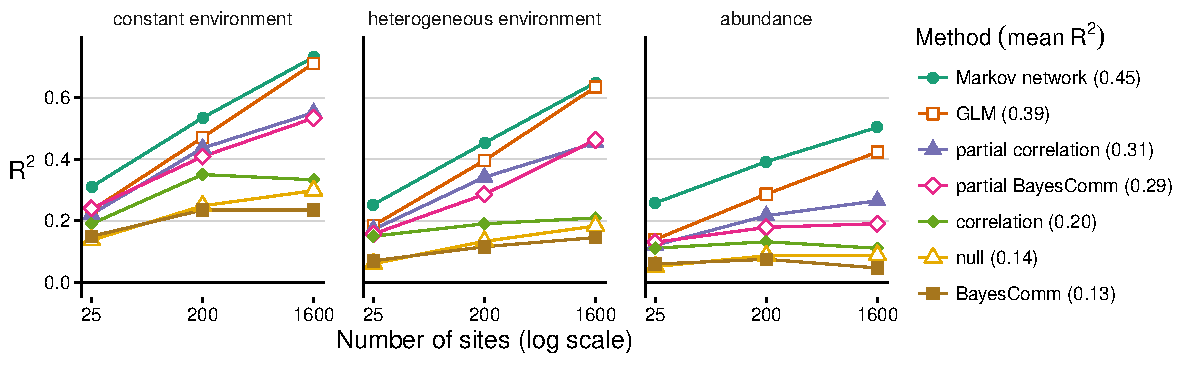
\includegraphics{figures/performance.pdf}
\caption{Proportion of variance in interaction coefficients explained by
each method versus number of sampled locations across the three
simulation types. For the null model (Pairs), two outliers with
\(|Z|>1000\) were manually adjusted to \(|Z|=50\) to mitigate their
detrimental influence on \(R^2\) (Appendix 5).}
\end{figure}

\begin{figure}[htbp]
\centering
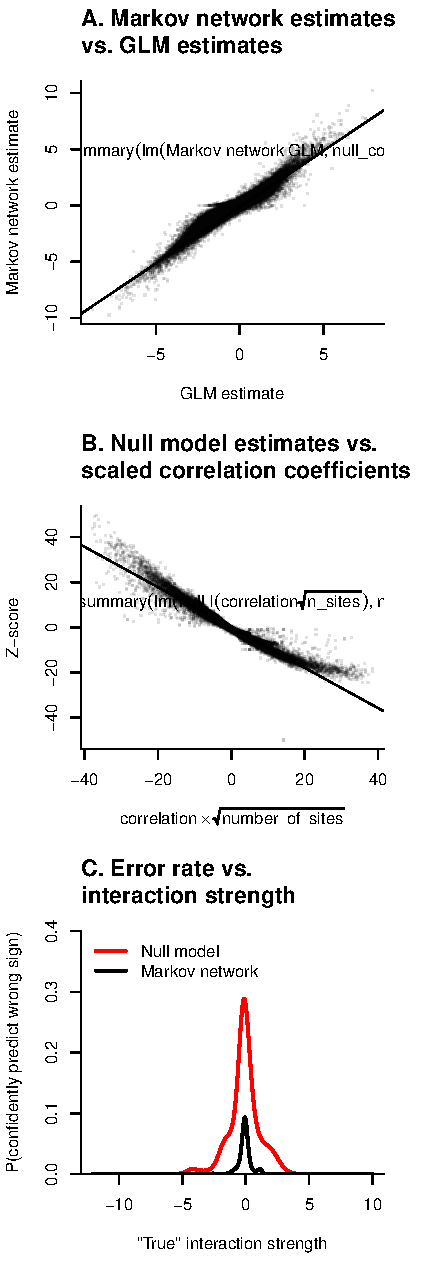
\includegraphics{figures/error_rates.pdf}
\caption{\textbf{A.} The Markov network's estimated interaction
coefficients were generally very similar to the GLM estimates.
\textbf{B.} The null model's estimates typically matched the (negative)
correlation coefficient, after controlling for landscape size.
\textbf{C.} For any given interaction strength, the null model was much
more likely to misclassify its sign with 95\% confidence than the Markov
network was.}
\end{figure}

Of the methods that did not control for indirect effects, Figure 3 shows
that simple correlation coefficients provided a more reliable indicator
of species' true interaction strengths than either the joint species
distribution model (BayesComm) or the null model (Pairs). The estimates
from these approaches were tightly correlated (after controlling for the
size of the landscape) suggesting that the null model only contains a
noisy version of the same information that could be obtained more easily
and interpretably with simple correlation coefficients (Figure 4B).

Finally, we can evaluate the models' statistical inferences (focusing on
the first two simulation types, for which the true interaction rates are
easiest to interpret). The Markov network's approximate Type I error
rate (defined here as the probability that 0 fell outside the 95\%
confidence interval for a pair of species where \(|\beta_{ij}|<0.1\))
depended on the simulation type: 0.02 for simulations that matched the
model's assumptions, versus 0.14 for simulations that included
environmental heterogeneity (see Appendix 4 for confidence interval
coverage across a range of \(\beta_{ij}\) values). The null model's Type
I error rates were 0.30 and 0.50 for the constant and heterogeneous
landscapes, respectively---far higher than the nominal 0.05 rate. Figure
4C shows, across a range of true interaction strengths, the probability
that the null model or the Markov network will predict the wrong sign of
the interaction with 95\% confidence. The null model makes such errors
more than 5 times as often as the Markov network, even though it only
reject the null hypothesis twice as often overall (Appendix 4). The
Markov network's errors were also more concentrated around 0, so it
never misclassified strong interactions like the null model did.

\noindent
\textbf{Discussion}

\noindent
The results presented above show that Markov networks can reliably
recover species' pairwise interactions from species composition data,
even for cases where environmental heterogeneity and indirect
interactions cause ecologists' typical null modeling approaches to
reliably fail. Partial covariances and generalized linear models can
both provide computationally efficient approximations, but with somewhat
lower accuracy (especially for typically-sized data sets with small
numbers of sites; Gotelli and Ulrich 2009). The difference in accuracy
may be larger for real data sets than for the simulated landscapes in
Figure 3, however; linear approximations to the Markov network make
larger errors when the interaction matrix is structured (e.g.~due to
guilds or trophic levels; Loh and Wainwright 2013). Similarly, the
separate generalized linear models for each species can severely overfit
in some cases (Lee and Hastie 2012). The full Markov network should thus
be preferred to the approximations when it is computationally tractable.

Compositional data only contains enough degrees of freedom to estimate
one interaction per species pair (Schmidt and Murphy 2012), so none of
these methods can identify the exact nature of the pairwise interactions
(e.g.~which species in a positively-associated pair is facilitating the
other). To estimate asymmetric interactions, such as commensalism or
predation, ecologists could use time series, behavioral observations,
manipulative experiments, or natural history. These other sources of
information could also be used to augment the likelihood function with a
more informative prior distribution, reducing ecologists' error and
uncertainty relative to Figure 3's results.

Despite their limitations, Markov networks have enormous potential to
improve ecological understanding. In particular, they make many fewer
errors than existing approaches, and can make precise statements about
the conditions where indirect interactions will overwhelm direct ones.
They also provide a simple answer to the question of how competition
should affect a species' overall prevalence, which has important
implications for community-level modeling (Strong et al. 1984).
Specifically, Equation 1 can be used to calculate the expected
prevalence of a species in the absence of biotic influences as
\(e^\alpha/(e^{0} + e^\alpha)\). Competition's effect on prevalence can
then be estimated by comparing this value with the observed prevalence
(e.g.~comparing Figure 2D with Figure 2C). This novel quantitative
result conflicts with most of our null models, which unreasonably assume
that prevalence would be the exactly same in the absence of competition
as it is in the observed data (Roughgarden 1983).

Markov networks---particularly the Ising model for binary networks---are
very well understood, having been studied for nearly a century (Cipra
1987). Tapping into this framework would thus allow ecologists to take
advantage of into a vast set of existing discoveries and techniques for
dealing with indirect effects, stability, and alternative stable states.
Numerous extensions to the basic network are possible as well. For
example, the states of the interaction network can be modeled as a
function of the local abiotic environment (Lee and Hastie 2012), which
would help incorporate networks of biotic interactions into species
distribution models (Pollock et al. 2014) and lead to a better
understanding of the interplay between biotic and abiotic effects on
community structure. Alternatively, models could allow one species to
alter the relationship between two other species (Tjelmeland and Besag
1998, cf Bruno et al. 2003).

Finally, the results presented here have important implications for
ecologists' continued use of null models for studying species
interactions. Null and neutral models can be useful for clarifying our
thinking (Harris et al. 2011, Xiao et al. 2015), but deviations from a
particular null model must be interpreted with care (Roughgarden 1983).
Even in small networks with three species, it may simply not be possible
to implicate specific ecological processes like competition by rejecting
a general-purpose null (Gotelli and Ulrich 2009), especially when the
test statistic is effectively just a correlation coefficient (Figure
4B). When the non-null backdrop is not controlled for, Type I error
rates can skyrocket, the apparent sign of the interaction can change,
and null models can routinely produce misleading inferences (Figure 1,
Figure 4C, Gotelli and Ulrich (2009)).

Controlling for indirect effects via simultaneous estimation of multiple
ecological parameters seems like a much more promising approach: to the
extent that the models' relative performance on real data sets is
similar to the range of results shown in Figure 3, scientists in this
field could often triple their explanatory power by switching from null
models to Markov networks (or increase it nearly as much with linear or
generalized linear approximations). Regardless of the methods ecologists
ultimately choose, controlling for indirect effects could clearly
improve our understanding of species' direct effects on one another and
on community structure.

\noindent \textbf{Acknowledgements:} This work benefited greatly from
discussions with A. Sih, M. L. Baskett, R. McElreath, R. J. Hijmans, A.
C. Perry, and C. S. Tysor. Additionally, A. K. Barner, E. Baldridge, E.
P. White, D. Li, D. L. Miller, N. Golding, N. J. Gotelli, C. F. Dormann,
and two anonymous reviewers provided very helpful feedback on the text.
This research was partially supported by a Graduate Research Fellowship
from the US National Science Foundation and by the Gordon and Betty
Moore Foundation's Data-Driven Discovery Initiative through Grant
GBMF4563 to E. P. White.

\setlength{\parindent}{0cm}

\noindent \textbf{References:}

\setlength{\parindent}{-1em} \setlength{\leftskip}{1em}
\setlength{\parskip}{0pt}

\hyperdef{}{refs}{\label{refs}}
\hyperdef{}{ref-albrechtux5fspatialux5f2001}{\label{ref-albrechtux5fspatialux5f2001}}
Albrecht, M., and N. J. Gotelli. 2001. Spatial and temporal niche
partitioning in grassland ants. Oecologia 126:134--141.

\hyperdef{}{ref-azaeleux5finferringux5f2010}{\label{ref-azaeleux5finferringux5f2010}}
Azaele, S., R. Muneepeerakul, A. Rinaldo, and I. Rodriguez-Iturbe. 2010.
Inferring plant ecosystem organization from species occurrences. Journal
of theoretical biology 262:323--329.

\hyperdef{}{ref-brunoux5finclusionux5f2003}{\label{ref-brunoux5finclusionux5f2003}}
Bruno, J. F., J. J. Stachowicz, and M. D. Bertness. 2003. Inclusion of
facilitation into ecological theory. Trends in Ecology \& Evolution
18:119--125.

\hyperdef{}{ref-cipraux5fintroductionux5f1987}{\label{ref-cipraux5fintroductionux5f1987}}
Cipra, B. A. 1987. An introduction to the Ising model. American
Mathematical Monthly 94:937--959.

\hyperdef{}{ref-connorux5fcheckeredux5f2013}{\label{ref-connorux5fcheckeredux5f2013}}
Connor, E. F., M. D. Collins, and D. Simberloff. 2013. The checkered
history of checkerboard distributions. Ecology 94:2403--2414.

\hyperdef{}{ref-diamondux5fislandux5f1975}{\label{ref-diamondux5fislandux5f1975}}
Diamond, J. M. 1975. The island dilemma: Lessons of modern biogeographic
studies for the design of natural reserves. Biological conservation
7:129--146.

\hyperdef{}{ref-faisalux5finferringux5f2010}{\label{ref-faisalux5finferringux5f2010}}
Faisal, A., F. Dondelinger, D. Husmeier, and C. M. Beale. 2010.
Inferring species interaction networks from species abundance data: A
comparative evaluation of various statistical and machine learning
methods. Ecological Informatics 5:451--464.

\hyperdef{}{ref-friedmanux5fsparseux5f2008}{\label{ref-friedmanux5fsparseux5f2008}}
Friedman, J., T. Hastie, and R. Tibshirani. 2008. Sparse inverse
covariance estimation with the graphical lasso. Biostatistics
9:432--441.

\hyperdef{}{ref-gelfandux5fmodellingux5f2005}{\label{ref-gelfandux5fmodellingux5f2005}}
Gelfand, A. E., A. M. Schmidt, S. Wu, J. A. Silander, A. Latimer, and A.
G. Rebelo. 2005. Modelling species diversity through species level
hierarchical modelling. Journal of the Royal Statistical Society: Series
C (Applied Statistics) 54:1--20.

\hyperdef{}{ref-gelmanux5fweaklyux5f2008}{\label{ref-gelmanux5fweaklyux5f2008}}
Gelman, A., A. Jakulin, M. G. Pittau, and Y.-S. Su. 2008. A Weakly
Informative Default Prior Distribution for Logistic and Other Regression
Models. The Annals of Applied Statistics 2:1360--1383.

\hyperdef{}{ref-gilpinux5ffactorsux5f1982}{\label{ref-gilpinux5ffactorsux5f1982}}
Gilpin, M. E., and J. M. Diamond. 1982. Factors contributing to
non-randomness in species Co-occurrences on Islands. Oecologia
52:75--84.

\hyperdef{}{ref-goldingux5fbayescommux5f2015}{\label{ref-goldingux5fbayescommux5f2015}}
Golding, N., and D. J. Harris. 2015. BayesComm: Bayesian Community
Ecology Analysis.

\hyperdef{}{ref-gotelliux5fempiricalux5f2009}{\label{ref-gotelliux5fempiricalux5f2009}}
Gotelli, N. J., and W. Ulrich. 2009. The empirical Bayes approach as a
tool to identify non-random species associations. Oecologia
162:463--477.

\hyperdef{}{ref-harrisux5frosaliaux5f2015}{\label{ref-harrisux5frosaliaux5f2015}}
Harris, D. J. 2015a. Rosalia: Exact inference for small binary Markov
networks. R package version 0.1.0. Zenodo.
http://dx.doi.org/10.5281/zenodo.17808.

\hyperdef{}{ref-harrisux5fgeneratingux5f2015}{\label{ref-harrisux5fgeneratingux5f2015}}
Harris, D. J. 2015b. Generating realistic assemblages with a Joint
Species Distribution Model. Methods in Ecology and Evolution.

\hyperdef{}{ref-harrisux5foccupancyux5f2011}{\label{ref-harrisux5foccupancyux5f2011}}
Harris, D. J., K. G. Smith, and P. J. Hanly. 2011. Occupancy is
nine-tenths of the law: Occupancy rates determine the homogenizing and
differentiating effects of exotic species. The American naturalist
177:535.

\hyperdef{}{ref-harrisux5fcontactux5f1974}{\label{ref-harrisux5fcontactux5f1974}}
Harris, T. E. 1974. Contact Interactions on a Lattice. The Annals of
Probability 2:969--988.

\hyperdef{}{ref-leeux5flearningux5f2012}{\label{ref-leeux5flearningux5f2012}}
Lee, J. D., and T. J. Hastie. 2012, May. Learning Mixed Graphical
Models.

\hyperdef{}{ref-levineux5fcompetitiveux5f1976}{\label{ref-levineux5fcompetitiveux5f1976}}
Levine, S. H. 1976. Competitive Interactions in Ecosystems. The American
Naturalist 110:903--910.

\hyperdef{}{ref-lewinux5fsantaux5f1983}{\label{ref-lewinux5fsantaux5f1983}}
Lewin, R. 1983. Santa Rosalia Was a Goat. Science 221:636--639.

\hyperdef{}{ref-lohux5fstructureux5f2013}{\label{ref-lohux5fstructureux5f2013}}
Loh, P.-L., and M. J. Wainwright. 2013. Structure estimation for
discrete graphical models: Generalized covariance matrices and their
inverses. The Annals of Statistics 41:3022--3049.

\hyperdef{}{ref-macarthurux5fpopulationux5f1958}{\label{ref-macarthurux5fpopulationux5f1958}}
MacArthur, R. H. 1958. Population ecology of some warblers of
northeastern coniferous forests. Ecology 39:599--619.

\hyperdef{}{ref-murphyux5fmachineux5f2012}{\label{ref-murphyux5fmachineux5f2012}}
Murphy, K. P. 2012. Machine Learning: A Probabilistic Perspective. The
MIT Press.

\hyperdef{}{ref-pollockux5funderstandingux5f2014}{\label{ref-pollockux5funderstandingux5f2014}}
Pollock, L. J., R. Tingley, W. K. Morris, N. Golding, R. B. O'Hara, K.
M. Parris, P. A. Vesk, and M. A. McCarthy. 2014. Understanding
co-occurrence by modelling species simultaneously with a Joint Species
Distribution Model (JSDM). Methods in Ecology and Evolution:n/a--n/a.

\hyperdef{}{ref-rux5fcoreux5fteamux5frux5f2015}{\label{ref-rux5fcoreux5fteamux5frux5f2015}}
R Core Team. 2015. R: A Language and Environment for Statistical
Computing. R Foundation for Statistical Computing, Vienna, Austria.

\hyperdef{}{ref-roughgardenux5fcompetitionux5f1983}{\label{ref-roughgardenux5fcompetitionux5f1983}}
Roughgarden, J. 1983. Competition and Theory in Community Ecology. The
American Naturalist 122:583--601.

\hyperdef{}{ref-schaferux5fcorpcorux5f2014}{\label{ref-schaferux5fcorpcorux5f2014}}
Schäfer, J., R. Opgen-Rhein, V. Zuber, M. Ahdesmäki, A. P. D. Silva, and
K. Strimmer. 2014. Corpcor: Efficient Estimation of Covariance and
(Partial) Correlation.

\hyperdef{}{ref-schmidtux5fmodelingux5f2012}{\label{ref-schmidtux5fmodelingux5f2012}}
Schmidt, M., and K. Murphy. 2012. Modeling Discrete Interventional Data
using Directed Cyclic Graphical Models. arXiv preprint arXiv:1205.2617.

\hyperdef{}{ref-strongux5fecologicalux5f1984}{\label{ref-strongux5fecologicalux5f1984}}
Strong, D. R., D. Simberloff, L. G. Abele, and A. B. Thistle. 1984.
Ecological communities: Conceptual issues and the evidence. Princeton
University Press.

\hyperdef{}{ref-tjelmelandux5fmarkovux5f1998}{\label{ref-tjelmelandux5fmarkovux5f1998}}
Tjelmeland, H., and J. Besag. 1998. Markov Random Fields with
Higher-order Interactions. Scandinavian Journal of Statistics
25:415--433.

\hyperdef{}{ref-veechux5fprobabilisticux5f2013}{\label{ref-veechux5fprobabilisticux5f2013}}
Veech, J. A. 2013. A probabilistic model for analysing species
co-occurrence. Global Ecology and Biogeography 22:252--260.

\hyperdef{}{ref-whittamux5fspeciesux5f1981}{\label{ref-whittamux5fspeciesux5f1981}}
Whittam, T. S., and D. Siegel-Causey. 1981. Species Interactions and
Community Structure in Alaskan Seabird Colonies. Ecology 62:1515--1524.

\hyperdef{}{ref-xiaoux5fstrongux5f2015}{\label{ref-xiaoux5fstrongux5f2015}}
Xiao, X., D. J. McGlinn, and E. P. White. 2015. A strong test of the
Maximum Entropy Theory of Ecology. The American Naturalist 185:E70--E80.
\end{flushleft}
\end{spacing}

\end{document}
